\documentclass{article}
\usepackage{amsmath,amssymb,graphicx,tikz}
\usepackage{hyperref}
\usepackage{tikz}
\usepackage{amsfonts}
\usepackage{amsmath}
\usepackage{listings}
\usetikzlibrary{fit}

\title{CSC263 Winter 2016, Assignment 2}
\author{Connor Peet \#1001088208}
\renewcommand{\today}{~}
\hypersetup{pdfpagemode=Fullscreen,
  colorlinks=true,
  linkfileprefix={}}
\begin{document}
\maketitle

\lstset{
    numbers=left
}

\begin{enumerate}
\item [1.] See figures 1 and 2 on the following page.
    \begin{figure}[p]
    \centering
    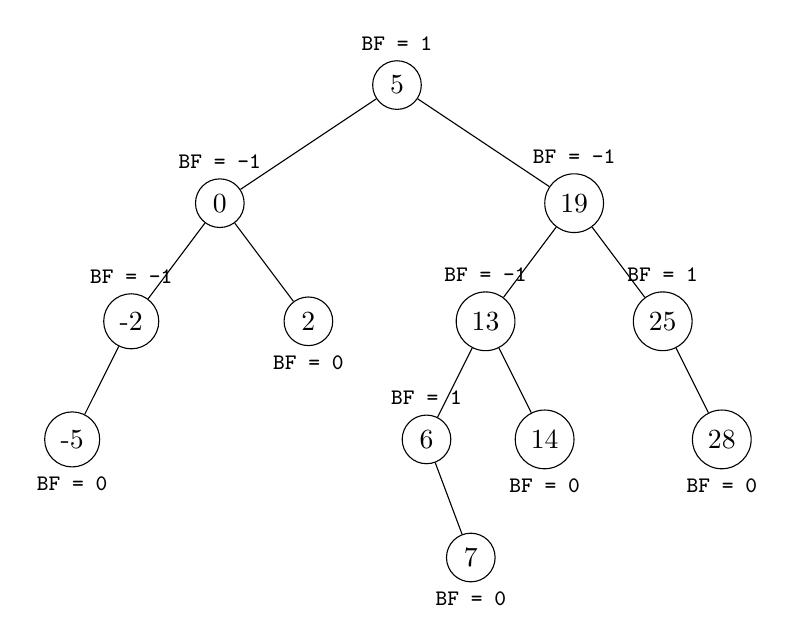
\begin{tikzpicture}[
        level/.style={sibling distance=45mm/#1, level distance = 15mm},
        every node/.style={align=center},
        label distance=0mm,
        every label/.style={text width=20mm, below},
    ]
    \tikzstyle{every label}=[font=\footnotesize]
    \node[circle,draw,label=\texttt{BF = 1}]{5}
        child{ node[circle,draw, label=\texttt{BF = -1}]{0}
            child{ node[circle,draw,label=\texttt{BF = -1}]{-2}
                child{ node[circle,draw,label=below:\texttt{BF = 0}]{-5} }
                child[missing]{}
            }
            child{ node[circle,draw,label=below:\texttt{BF = 0}]{2} }
        }
        child{ node[circle,draw,label=\texttt{BF = -1}]{19}
            child{ node[circle,draw,label=\texttt{BF = -1}]{13}
                child{ node[circle,draw,label=\texttt{BF = 1}]{6}
                    child[missing]{}
                    child{ node[circle,draw,label=below:\texttt{BF = 0}]{7} }
                }
                child{ node[circle,draw,label=below:\texttt{BF = 0}]{14} }
            }
            child{ node[circle,draw,label=\texttt{BF = 1}]{25}
                child[missing]{}
                child{ node[circle,draw,label=below:\texttt{BF = 0}]{28} }
            }
        };
    \end{tikzpicture}
    \caption{The resulting AVL tree $T$.}
    \end{figure}

    \begin{figure}[p]
    \centering
    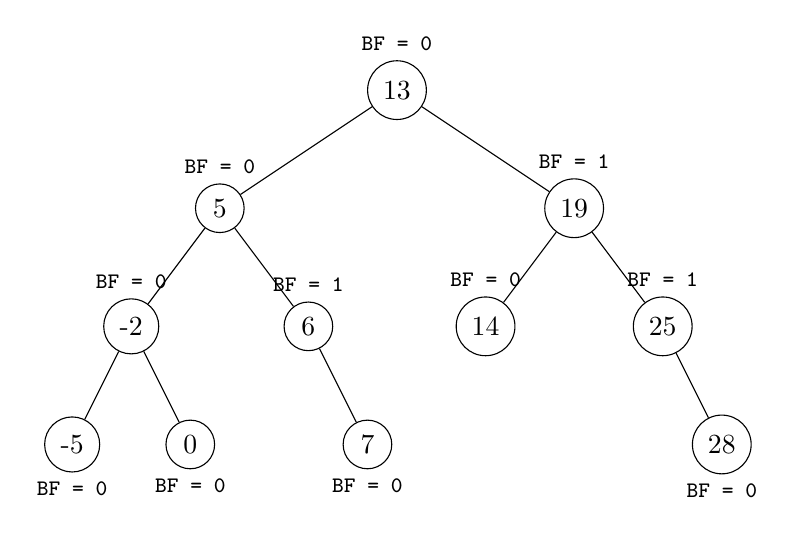
\begin{tikzpicture}[
        level/.style={sibling distance=45mm/#1, level distance = 15mm},
        every node/.style={align=center},
        label distance=0mm,
        every label/.style={text width=20mm, below},
    ]
    \tikzstyle{every label}=[font=\footnotesize]
    \node[circle,draw,label=\texttt{BF = 0}]{13}
        child{ node[circle,draw, label=\texttt{BF = 0}]{5}
            child{ node[circle,draw,label=\texttt{BF = 0}]{-2}
                child{ node[circle,draw,label=below:\texttt{BF = 0}]{-5} }
                child{ node[circle,draw,label=below:\texttt{BF = 0}]{0} }
            }
            child{ node[circle,draw,label=\texttt{BF = 1}]{6}
                child[missing]{}
                child{ node[circle,draw,label=below:\texttt{BF = 0}]{7} }
            }
        }
        child{ node[circle,draw,label=\texttt{BF = 1}]{19}
            child{ node[circle,draw,label=\texttt{BF = 0}]{14} }
            child{ node[circle,draw,label=\texttt{BF = 1}]{25}
                child[missing]{}
                child{ node[circle,draw,label=below:\texttt{BF = 0}]{28} }
            }
        };
    \end{tikzpicture}
    \caption{$T$ after deleting $2$ and executing the necessary rotations.}
    \end{figure}

\item [2.] First we define a \texttt{pull\_root} function that takes removes and returns either the smallest element of $B_2$ or the largest element of $B_1$.
\begin{lstlisting}
def pull_root(B1, B2):
    node_b1 = B1.root
    node_b2 = B2.root

    while True:
        if node_b1.right == nil:
            if node_b1.parent != nil:
                node_b1.parent.right = nil
            return node_b1

        elif node_b2.left == nil:
            if node_b2.parent != nil:
                node_b2.parent.left = nil
            return node_b2

        node_b1 = node_b1.right
        node_b2 = node_b2.left
\end{lstlisting}

    The function to merge the trees is a trivial extension of \texttt{pull\_root}:
\begin{lstlisting}
def merge(B1, B2):
    root = pull_root(B1, B2)
    root.left = B1
    root.right = B2
    B1.parent = root
    B2.parent = root
\end{lstlisting}

    In this function, we're running down the right-most subtrees of $B_1$ and left-most subtrees of $B_2$ until we get to the leaf of either. This relies on the invariants of BSTs. When the node is found, it's removed from its parent and returned. The while loop will run at most $min\{h_1, h_2\}$ times--it loops down $B_1$ and $B_2$ and aborts as soon as it reaches a leaf of either--and each function inside the loop takes a constant time, so the function is in $O(min\{h_1, h_2\})$. \\

    The leaf that's removed and returned is either the largest item in $B_1$ or the smallest item in $B_2$. In both cases this item can be assigned to the root of the tree while preserving the BST property. \\

    The maximum height change occurs when the removed leaf was not the single deepest node out of both trees. When this occurs, the height of the new tree $T$ is $max\{h_1, h_2\} + 1$ as the result of inserting a new root above the subtrees. If this is not the case, then height of $T$ will equal $max\{h_1, h_2\}$.

\item [3.] To create this `rolling median' I'll use two heaps. The first heap, $H_1$ is a max-heap and the second $H_2$ is a min-heap. The following algorithms can be used to insert and find the median of heaps $H_1$ and $H_2$. For conciseness, algorithms already defined in the textbook (heap insert and extraction) are not shown.
\begin{lstlisting}
def median(H1, H2):
    if H1.size > H2.size:
        return H1.root
    else:
        return (H1.root + H2.root) / 2

def insert(H1, H2, x):
    if H1.size == 0 or x <= H1.root:
        H1.insert(x)
    else:
        H2.insert(x)

    if H2.size > H1.size:
        H1.insert(H2.extract_root())
    elif H1.size > H2.size + 1:
        H2.insert(H1.extract_root())

def median_list(A):
    H1 = new Heap()
    H2 = new Heap()

    M = []
    for i in [1..n]:
        insert(H1, H2, A[i])
        M[i] = median(H1, H2)

    return M

\end{lstlisting}
    Notes on correctness of \texttt{median}, keeping in mind min and max heap properties:
    \begin{enumerate}
        \item It's invariant that $H_1$ always has either $H_2.size$ or $H_2.size + 1$ items. This is maintained in lines 13 through 16 of \texttt{insert}; items are rebalanced to ensure this is the case.
        \item By (a), $H_1.size$ is larger than $H_2.size$ only if $i$ is odd.
        \item It's also invariant that all items in $H_1$ are less than or equal to all items in $H_2$:
            \begin{itemize}
            \item The first item is inserted in $H_1$, so the invariant holds.
            \item For $i > 1$, the \textit{i}th item is inserted in $H_1$ iff it's less than or equal to the root, which is greater than all its other elements due to the max-heap property. Otherwise, it's inserted into $H_2$, as it's greater than the largest element in $H_1$.
            \item When a rebalance happens (lines 13 to 16), either the largest element from $H_1$ is moved to $H_2$, or the smallest element is moved from $H_2$ to $H_1$. In both cases, the invariant holds.
            \end{itemize}
        \item $H_1.size + H_2.size = i$
        \item By the above, when looking at $A[1..i]$ in sorted order:
            \begin{itemize}
            \item If $i$ is odd, the root of $H_1$ is preceded by the $(i - 1) / 2$ children in $H_1$ and proceeded by the remaining $(i - 1) / 2$ nodes in $H_2$. Then it is of rank $(i + 1) / 2$, so we return it correctly as the median.
            \item If $i$ is even, the two roots are preceded by the $i / 2 - 1$ children in $H_1$ and proceeded by the $i / 2 - 1$ children in $H_2$. Then they are of rank $i / 2$ and $i / 2 + 1$, so their average is returned correctly as the median.
            \end{itemize}
    \end{enumerate}
    The median is called as items are sequentially inserted into the heaps by \texttt{median\_list} and appended to $M$. From the above reasoning and pseudo-code, it's evident that $M[i]$ is the correct median of $A[1..i]$, so the output will be correct. \\

    From the textbook, we know that the running time of heap extraction and insertion is in $O(\log n)$. Each call to \texttt{insert} runs at most two insertions and one extraction, and calls to \texttt{median} run in constant time. We call \texttt{median} and \texttt{insert} $n$ times in lines 24 and 25 of \texttt{median\_list}, which otherwise runs in constant time. Therefore the algorithm runs in $O(n \log n)$ time.

\end{enumerate}
\end{document}
